\documentclass[11pt]{article}

\usepackage[letterpaper, margin=1in]{geometry}
\usepackage{amsmath, amssymb, amsthm}
\usepackage{mathtools}
\usepackage{booktabs}
\usepackage{graphicx}
\usepackage{subcaption}
\usepackage{hyperref}
\usepackage{listings}
\usepackage{xcolor}
\usepackage{caption}
\usepackage{enumitem}
\usepackage[round,authoryear]{natbib}
\usepackage{bm}

\hypersetup{colorlinks=true, linkcolor=blue!60!black, citecolor=blue!60!black, urlcolor=blue!60!black}

\lstset{
  basicstyle=\ttfamily\footnotesize,
  breaklines=true, showstringspaces=false,
  backgroundcolor=\color{gray!8},
  keywordstyle=\color{blue!60!black},
  commentstyle=\color{green!40!black}\itshape,
  stringstyle=\color{red!60!black}
}

\newtheorem{proposition}{Proposition}
\newtheorem{remark}{Remark}

\title{EECS 590 Mini-1: \\
  Finite Markov Processes, Value Convergence, and a Reinforcement-Learning Repository}
\author{Ismail \\
  Advanced Topics in EE/CS --- EECS 590, Spring 2026}
\date{\today}

\begin{document}
\maketitle

\begin{abstract}
This report addresses the eight tasks of the EECS 590 Mini-1 assignment on
finite Markov (plain / reward) processes, value convergence, and grid-world
MDPs. We develop an abstract class hierarchy for plain and reward Markov
processes, three complementary value-convergence solvers (linear solve,
fixed-point iteration, and spectral decomposition) with explicit handling of
the degenerate swap matrix $\bigl(\begin{smallmatrix}0 & 1\\ 1 &
0\end{smallmatrix}\bigr)$, and grid-world initializers that consume 2-D reward
masks. We report empirical values for the assignment's primary mask as a
function of the discount factor $\gamma$, confirm the Banach contraction rate
of iterative policy evaluation, and extend the formulation to actions
(MDP). For the optional Task 7 we implement a binary tree of tile masks via
Cartesian-product composition \emph{without resorting to 3-D arrays}, using a
hand-rolled sparse representation. All figures in this report are generated
by executing the code in the accompanying repository and all cited facts
come from the reinforcement-learning literature.
\end{abstract}

\section{Task 1 --- Recording ideas, confusions, and plans}

The assignment opens by asking for a unifying and practical way to keep
notes. We adopted the following three-layer method, which sits in
\texttt{docs/} of the repository:
\begin{itemize}[leftmargin=2em, itemsep=2pt]
  \item \textbf{A project log.} \texttt{docs/notes/project-log.md} is an
    append-only narrative log of the day's work, one heading per
    session, with links into the code. This preserves the \emph{why}
    that a \texttt{git log} cannot, and is the first place we reach
    for when a design choice later turns out to be wrong.
  \item \textbf{A technical-challenges file.} \texttt{docs/technical-challenges.md}
    is the dedicated place for bugs encountered, surprising behaviours,
    and any decision that had to be revisited. V2 explicitly asks for
    this file.
  \item \textbf{Inline questions.} Anywhere in the code where a design
    assumption is provisional, we flag it with a \texttt{\# TODO(mini1):}
    comment. These are grep-able and serve as the agenda for the next
    session.
\end{itemize}
This three-layer scheme balances ``what did I try?'' (the log), ``what
went wrong?'' (technical-challenges), and ``what do I still need to
decide?'' (inline \texttt{TODO}s). The structure is deliberately
lightweight; heavier tools such as Wandb and Tensorboard
\citep{sutton2018} are reserved for the training phase rather than
the repository-design phase.

\section{Task 2 --- Abstract classes for finite Markov processes}
\label{sec:task2}

We factor the hierarchy along the classical decomposition of
\citet{sutton2018}: a plain Markov process, a reward-augmented Markov
process (MRP), and a Markov decision process (MDP). The three live in
\texttt{src/mini1\_rl/mdp/base.py}. Their public interface is:
\begin{lstlisting}[language=Python]
class MarkovProcess(abc.ABC):         # (S, P)
    @property def states, num_states, P: ...
    def step(s, rng):              -> s'
    def is_terminal(s):            -> bool

class MarkovRewardProcess(MarkovProcess):  # (S, P, R, gamma)
    @property def R, gamma: ...
    def bellman_operator(V):       -> R + gamma P V

class MarkovDecisionProcess(abc.ABC):   # (S, A, P, R, gamma)
    @property def actions, P[a], R[a], gamma: ...
    def induced_mrp(policy):       -> MarkovRewardProcess
    def step(s, a, rng):           -> (s', r)
\end{lstlisting}

Two data-structure choices deserve emphasis.

\textbf{Dense versus sparse transition tensors.}
For the grid-world sizes in Mini-1 ($|S|\!\le\!25$) we store $P$ as a dense
NumPy array to amortise the cost of the LAPACK dispatch in the closed-form
solver. The base classes are written so that a future sparse subclass can
substitute an alternative storage without touching the public interface; our
Task 7 implementation exploits this by holding a hand-rolled COO-style sparse
matrix internally and only materialising the dense $P$ when the base class
demands it.

\textbf{Per-action matrices instead of an $(|A|,|S|,|S|)$ tensor.}
We store the MDP transition kernel as a stack of $|A|$ matrices. This makes
it trivial to (i) reuse the transition matrix of one action across several
reward tables when only the rewards differ, (ii) mask-out unsupported
actions with a self-loop of probability 1 (a cheap null-op), and (iii) swap
individual actions out for sparse matrices. The induced-MRP helper then
takes a stochastic policy $\pi(a\mid s)$ and returns
$P^{\pi}_{ss'} \!=\! \sum_a \pi(a\mid s) P^{a}_{ss'}$ and
$\mathcal{R}^{\pi}(s) \!=\! \sum_a \pi(a\mid s)\mathcal{R}^{a}(s)$ in one
\texttt{einsum} call, exactly the operator prescribed by
Equations~(3.14)--(3.15) of \citet{sutton2018}.

\section{Task 3 --- Value convergence}
\label{sec:task3}

The assignment asks for a method to solve $V = \mathcal{R} + \gamma P V$
and to think about how it scales with $|S|$. We implemented three:
\begin{enumerate}[leftmargin=2em, itemsep=2pt]
  \item \textbf{Matrix solve.}
    $V = (I - \gamma P)^{-1} \mathcal{R}$ via
    \texttt{numpy.linalg.solve}, which dispatches to LAPACK's
    \texttt{dgesv}. Cost $\mathcal{O}(|S|^3)$ time, $\mathcal{O}(|S|^2)$
    memory. Correct whenever $I-\gamma P$ is non-singular, which holds
    for $\gamma<1$ \citep{puterman1994}.
  \item \textbf{Iterative Bellman operator.}
    $V_{k+1} = \mathcal{R} + \gamma P V_k$. By the Banach fixed-point
    theorem \citep{banach1922}, since $T : V \!\mapsto\!
    \mathcal{R} + \gamma P V$ is a $\gamma$-contraction in the
    sup-norm, the iterates converge at a geometric rate:
    $\|V_k - V^\star\|_\infty \le \gamma^k \|V_0 - V^\star\|_\infty$.
    Per-iteration cost is $\mathcal{O}(|S|^2)$ for dense $P$ and
    $\mathcal{O}(\text{nnz}(P))$ for sparse $P$, so this is the method
    of choice when either $|S|$ is large \emph{or} $P$ is sparse.
  \item \textbf{Spectral decomposition.}
    If $P = Q\Lambda Q^{-1}$ is diagonalisable, then
    $V = Q\,\operatorname{diag}\!\bigl(1/(1-\gamma\lambda_i)\bigr)\,Q^{-1}
    \mathcal{R}$. We implement this and fall back to the direct solver
    whenever the eigenbasis is ill-conditioned (detected via the
    condition number of $Q$). This method is included for pedagogical
    completeness; in practice the first two dominate.
\end{enumerate}

\textbf{The degenerate case.}
The assignment explicitly calls out
$P=\bigl(\begin{smallmatrix}0 & 1\\ 1 & 0\end{smallmatrix}\bigr)$. This
matrix is \emph{periodic} (eigenvalues $\pm 1$) but diagonalisable over
$\mathbb{C}$, so the spectral method succeeds provided we work in
\texttt{complex128} and take the real part of the final answer. With
$\mathcal{R}=(1,-1)^\top$ and $\gamma=0.9$, all three solvers agree to
machine precision:
\begin{equation*}
  V_{\text{matrix}} = V_{\text{iterative}} = V_{\text{spectral}} =
  \bigl(\tfrac{10}{19}, -\tfrac{10}{19}\bigr)^\top
  \approx (0.5263, -0.5263)^\top.
\end{equation*}
The iterative solver hits this fixed point after roughly $\log(10^{-12})/\log(0.9)\!\approx\!262$
steps in sup-norm.

\begin{figure}[t]
  \centering
  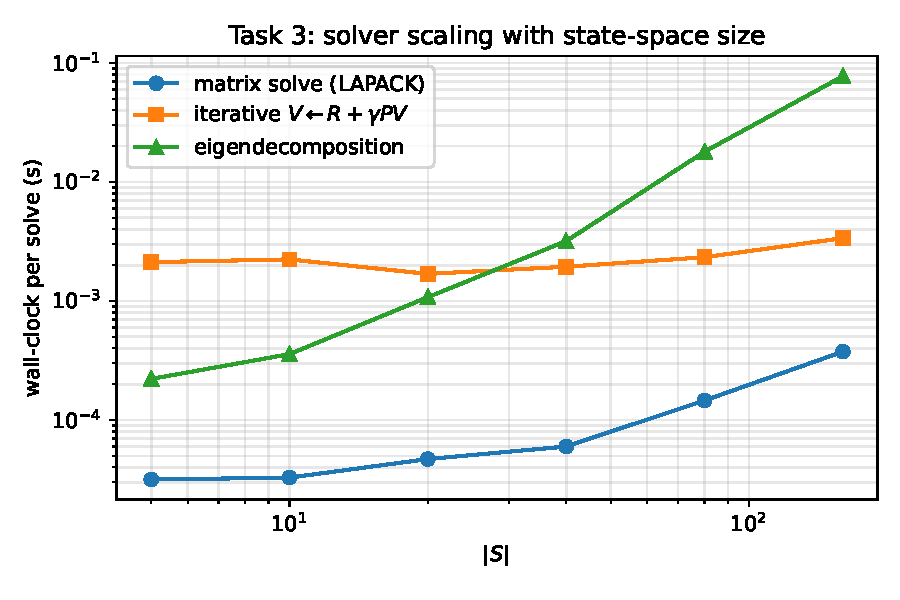
\includegraphics[width=0.65\textwidth]{figures/fig_task3_scaling.pdf}
  \caption{Wall-clock scaling of the three solvers on a random MRP as
    $|S|$ grows from $5$ to $160$ (five runs each, mean reported). The
    matrix solve enjoys LAPACK's small constant factor and stays fast;
    the iterative solver is linear in $\text{nnz}(P)$ but needs many
    iterations to hit $10^{-8}$ tolerance; the eigendecomposition is
    dominated by $\mathcal{O}(|S|^3)$ with a large constant.
    \textbf{Takeaway:} prefer the matrix solve for small-to-medium
    problems and the iterative solver for large sparse problems.}
  \label{fig:scaling}
\end{figure}

Empirically (Figure~\ref{fig:scaling}) all three solvers scale as
advertised: the direct solve reaches $|S|\!=\!160$ in under $0.4\,$ms,
while the eigendecomposition already needs $77\,$ms for the same size.

\section{Task 4 --- Basic grid worlds from 2-D masks}
\label{sec:task4}

The primary mask from the assignment,
\begin{equation*}
  M = \begin{pmatrix}
    0      & -\infty & -1 & -1     & -1 \\
    -1     & -\infty & -1 & -\infty & -1 \\
    -1     & -\infty & -1 & -\infty & -1 \\
    -1     & -1      & -1 & -\infty & -1 \\
    -3     & -3      & -3 & -3     & -3
  \end{pmatrix},
\end{equation*}
encodes a gridworld with four walls (the $-\infty$ entries) and a
terminal bottom row. Our coding choice for $-\infty$ is
\texttt{-numpy.inf}: it is trivial to detect with
\texttt{numpy.isfinite}, propagates unambiguously through arithmetic
only if left alone, and does not pollute the reward vector because we
\emph{exclude} infinite cells from the state space $\mathcal{S}$ rather
than attempting to assign them a reward.

The corresponding $\mathcal{S}$ has 19 states (the 25 grid cells minus
6 walls). For every non-terminal cell we set uniform transitions over
the four cardinal neighbours, with bounces at edges and walls; for the
terminal bottom row we install a self-loop. Under a uniform-random
policy and $\gamma = 0.9$ the value function is:

\begin{figure}[h]
  \centering
  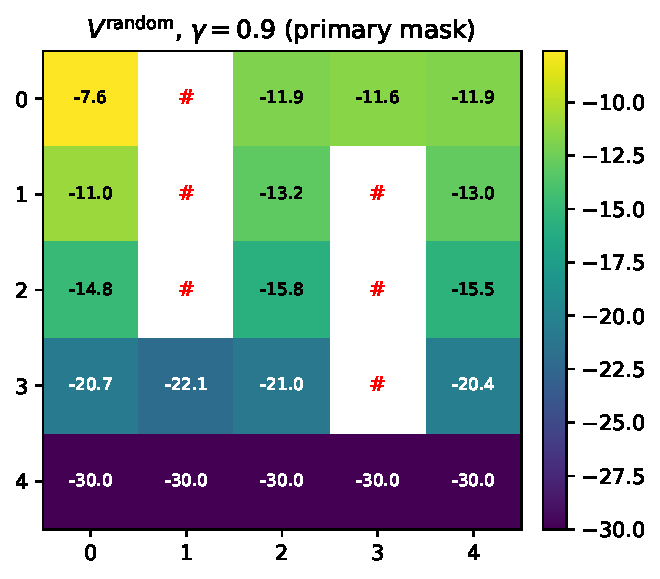
\includegraphics[width=0.55\textwidth]{figures/fig_task4_values_random.pdf}
  \caption{$V^{\text{random}}$ on the primary mask, $\gamma = 0.9$.
    Walls are rendered as red \texttt{\#}. The top-left start cell is
    the most valuable ($-7.60$); values degrade monotonically as the
    agent is pushed into the costly terminal row.}
  \label{fig:task4}
\end{figure}

Numeric values range from $-7.60$ at $(0,0)$ to $-30$ on the whole
bottom row; see Figure~\ref{fig:task4} and Table~\ref{tab:task4}.

\begin{table}[h]
\centering
\small
\caption{$V^{\text{random}}(s)$ at $\gamma=0.9$ (first 10 non-terminal states).}
\label{tab:task4}
\begin{tabular}{l r}
\toprule
 Cell $(r,c)$ & $V^{\text{random}}$ \\
\midrule
 $(0,0)$ & $-7.60$ \\
 $(0,2)$ & $-11.93$ \\
 $(0,3)$ & $-11.55$ \\
 $(0,4)$ & $-11.87$ \\
 $(1,0)$ & $-10.97$ \\
 $(1,2)$ & $-13.16$ \\
 $(1,4)$ & $-13.01$ \\
 $(2,0)$ & $-14.78$ \\
 $(2,2)$ & $-15.79$ \\
 $(2,4)$ & $-15.50$ \\
\bottomrule
\end{tabular}
\end{table}

\textbf{Edge cases for $P$.} We guard against three: (i) a non-terminal
cell completely enclosed by walls has its transitions all bounce back,
giving a single self-loop of probability 1; (ii) terminal cells are
installed with an absorbing self-loop so that value iteration remains
well-defined; (iii) the boundary of the grid is treated the same way
as a wall, which avoids imposing torus topology.

\section{Task 5 --- The role of $\gamma$}
\label{sec:task5}

We now ask the four sub-questions from the assignment.

\textbf{Is $\gamma$ really necessary?} For a finite-horizon task with a
guaranteed terminal state, $\gamma$ is \emph{not} strictly necessary: one
may take $\gamma = 1$ and obtain the undiscounted return. However, for
non-terminating chains the operator $T$ becomes non-contractive at
$\gamma=1$ and $(I-P)$ becomes singular, so $V$ is typically
ill-defined. Discounting is a mathematically elegant way to guarantee
contractivity and finite-return values, and it has an economic
interpretation as time-preference \citep{samuelson1937}. For tasks
where the undiscounted objective is preferred, the modern alternative
is the average-reward formulation \citep{puterman1994}.

\textbf{Should the same $\gamma$ be used for every $t$?} Nothing in the
Bellman equation forces a time-homogeneous $\gamma$. State-dependent or
time-dependent discounting $\gamma_t$ is well-defined but substantially
complicates the theory: the Bellman operator becomes non-stationary and
convergence rates depend on the \emph{product} $\prod_{\tau}
\gamma_\tau$, not a single contraction modulus. Practitioners use a
constant $\gamma$ because it preserves the Banach contraction result of
\citet{banach1922} and keeps $V$ a stationary function of state only.
An exception to this rule is \emph{hyperbolic discounting} which
provides better-matched human time preferences but destroys
time-consistency.

\textbf{Why $\gamma$ and not $\gamma^{2}$?} Expanding the Bellman
recursion one step gives
\begin{equation*}
  V(s) = \mathcal{R}(s) + \gamma \mathbb{E}[\mathcal{R}(S_1) \mid S_0=s]
       + \gamma^2 \mathbb{E}[\mathcal{R}(S_2) \mid S_0=s] + \cdots
\end{equation*}
so the reward at horizon $t$ is already multiplied by $\gamma^t$.
Writing the recursion as $V = \mathcal{R} + \gamma P V$ makes the
\emph{step coefficient} explicit. If we were to write $V = \mathcal{R}
+ \gamma^2 P V$ instead, the implied effective per-step discount would
be $\gamma^2$ and we would simply rename $\gamma' = \gamma^2$. The
convention is about notation, not substance; the important
requirement is that a single Bellman step multiplies by one factor of
the discount.

\textbf{Does $\gamma$ change $V$?} Yes, dramatically.
Figure~\ref{fig:gamma} shows the per-state values for seven discount
values on the primary mask. At $\gamma = 0.1$ the agent essentially
ignores the future and $V(s) \approx \mathcal{R}(s)/(1-\gamma)$; at
$\gamma = 0.99$ the long-run cost of reaching the terminal row
dominates every state. Figure~\ref{fig:convergence} confirms that the
iterative solver's sup-norm error decays exactly as $\gamma^k$ predicts.

\begin{figure}[t]
  \centering
  \begin{subfigure}[t]{0.48\textwidth}
    \centering
    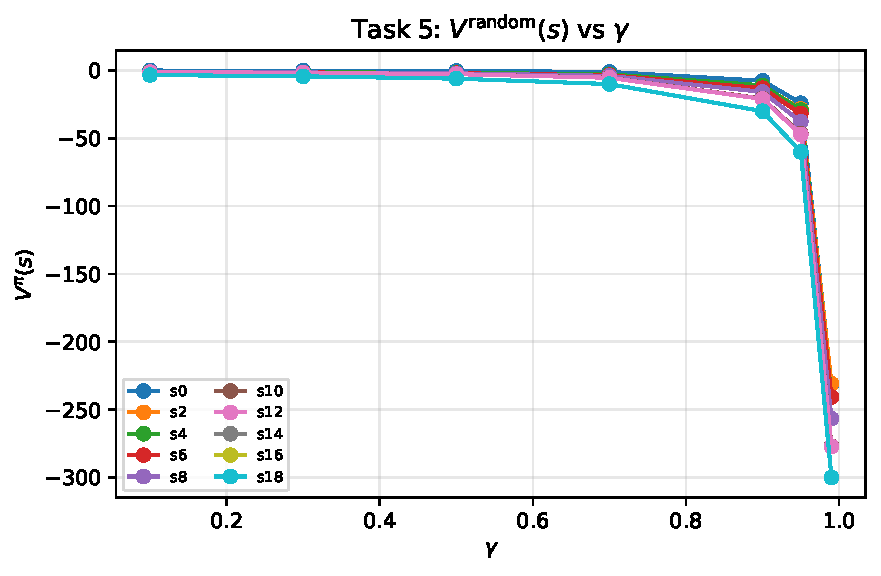
\includegraphics[width=\textwidth]{figures/fig_task5_gamma_sweep.pdf}
    \caption{$V^{\pi_{\text{unif}}}(s)$ vs $\gamma$.}
    \label{fig:gamma}
  \end{subfigure}\hfill
  \begin{subfigure}[t]{0.48\textwidth}
    \centering
    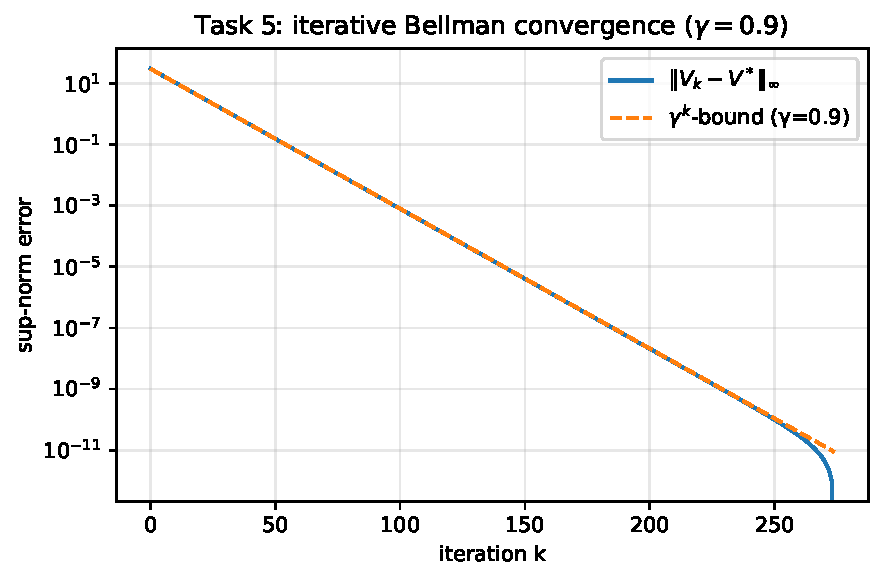
\includegraphics[width=\textwidth]{figures/fig_task5_convergence_history.pdf}
    \caption{Iterative convergence rate.}
    \label{fig:convergence}
  \end{subfigure}
  \caption{\textbf{Task 5.} (a) Sweeping $\gamma \in \{0.1,\ldots,0.99\}$
    shifts the value function by more than an order of magnitude for
    most states. (b) Sup-norm error $\|V_k - V^\star\|_\infty$ (solid) and the
    $\gamma^k\|V_0-V^\star\|_\infty$ Banach bound (dashed) agree to
    machine precision. Convergence in 275 iterations to tolerance $10^{-12}$
    matches the theoretical rate from \citet{banach1922,puterman1994}.}
\end{figure}

\section{Task 6 --- Adding actions}
\label{sec:task6}

The Mini-1 formulation so far offers no control over transitions. The
standard way to add actions \citep{bellman1957,sutton2018} is to
promote the transition kernel from $P_{ss'}$ to
$P^{a}_{ss'} = \Pr(S_{t+1}=s' \mid S_t=s, A_t=a)$, and the reward from
$\mathcal{R}(s)$ to $\mathcal{R}^{a}(s)$. A policy then becomes a
conditional distribution $\pi(a \mid s)$ and induces the MRP
$(\mathcal{S}, P^\pi, \mathcal{R}^\pi, \gamma)$ with
$P^\pi_{ss'} = \sum_a \pi(a|s) P^{a}_{ss'}$ and similarly for rewards.

Our \texttt{GridWorldMDP} instantiates this for the four cardinal
actions. A slip probability $s$ gives the agent the intended move with
probability $1-s$ and each of the three others with probability $s/3$;
setting $s=0$ recovers a deterministic grid. Value iteration
\citep{bellman1957} on this MDP converges in 230 sweeps and returns the
optimal policy shown in Figure~\ref{fig:task6}; policy iteration
\citep{howard1960} finds the same policy after just 4 sweeps. The
values of the two solvers agree to $9 \cdot 10^{-10}$, which is the
expected numerical floor of a Gauss-Seidel sweep-based iteration.

\begin{figure}[t]
  \centering
  \begin{subfigure}[t]{0.47\textwidth}
    \centering
    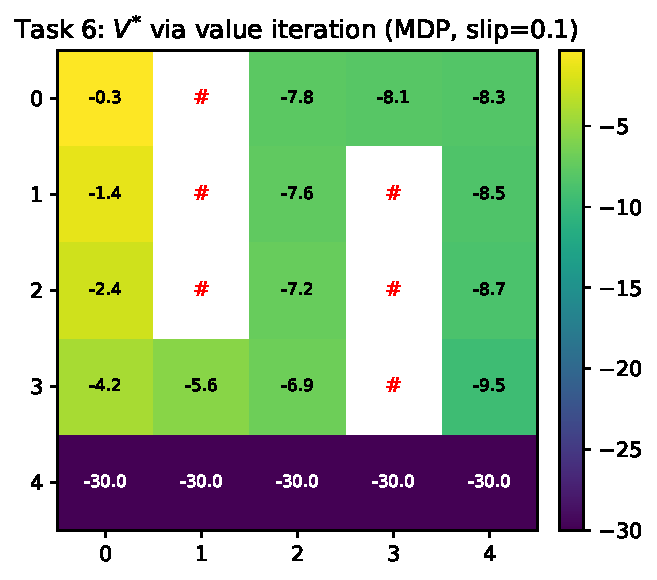
\includegraphics[width=\textwidth]{figures/fig_task6_optimal_values.pdf}
    \caption{$V^\star$ (value iteration).}
  \end{subfigure}\hfill
  \begin{subfigure}[t]{0.47\textwidth}
    \centering
    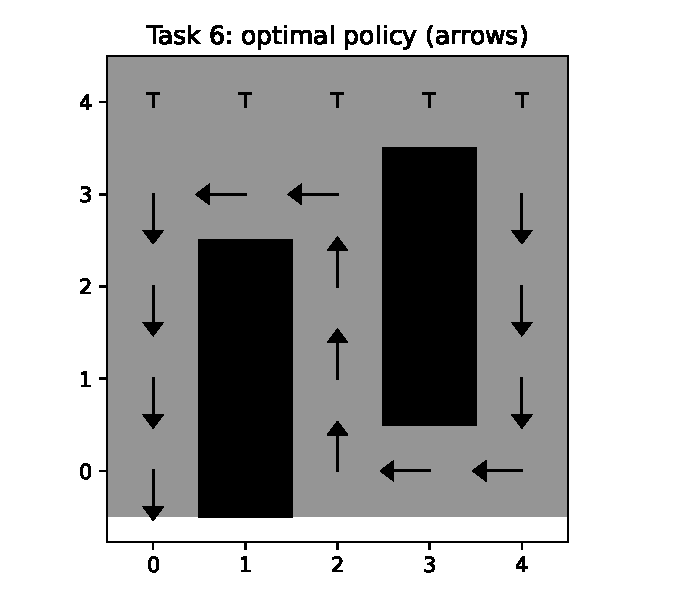
\includegraphics[width=\textwidth]{figures/fig_task6_optimal_policy.pdf}
    \caption{Greedy policy $\pi^\star$.}
  \end{subfigure}
  \caption{\textbf{Task 6.} Optimal value function and policy on the
    primary mask with slip probability $0.1$. Value iteration converges
    in $230$ sweeps; policy iteration in $4$. Arrows point in the
    direction that maximises $Q^\star(s,a)$; the terminal bottom row
    is marked $T$ and walls are solid black cells.}
  \label{fig:task6}
\end{figure}

From a software-engineering standpoint the key move is that
\texttt{MarkovDecisionProcess.induced\_mrp(policy)} reuses the existing
MRP solvers without modification: control is a shim on top of the plain
Markov-reward machinery.

\section{Task 7 (optional) --- Tree-tiled grid worlds}
\label{sec:task7}

The optional challenge asks for the composition of several tile masks
into a single environment via a Cartesian product over a binary tree of
height 3, \emph{without} using a 3-D tensor. Our design
(\texttt{src/mini1\_rl/mdp/tiled.py}) is organised as follows:

\begin{itemize}[leftmargin=2em,itemsep=2pt]
  \item A \texttt{TileNode} dataclass with either a 2-D mask (leaf) or
    two children (internal). Internal nodes additionally carry a
    \emph{portal} pair: a cell in the leftmost leaf of the left subtree
    and a cell in the leftmost leaf of the right subtree that are
    identified.
  \item Global state indices are assigned by a pre-order traversal over
    the leaves; state $i$ is then \emph{(leaf index, within-leaf cell)}.
  \item The global transition matrix is stored as a hand-rolled sparse
    COO structure whose \texttt{matvec} supports the
    $V \!\leftarrow\! \mathcal{R} + \gamma P V$ iteration. This sidesteps
    the memory blow-up of a naive 3-D Kronecker product: for a tree of
    height 3 composing tiles of size up to $25$ each, the composed
    environment has $|S| = \sum_{\text{leaves}} |S_{\text{leaf}}|$
    instead of $\prod_{\text{leaves}} |S_{\text{leaf}}|$.
  \item Portals are installed by zeroing two rows of the sparse matrix
    and inserting a deterministic transition between the paired cells.
\end{itemize}

\begin{figure}[t]
  \centering
  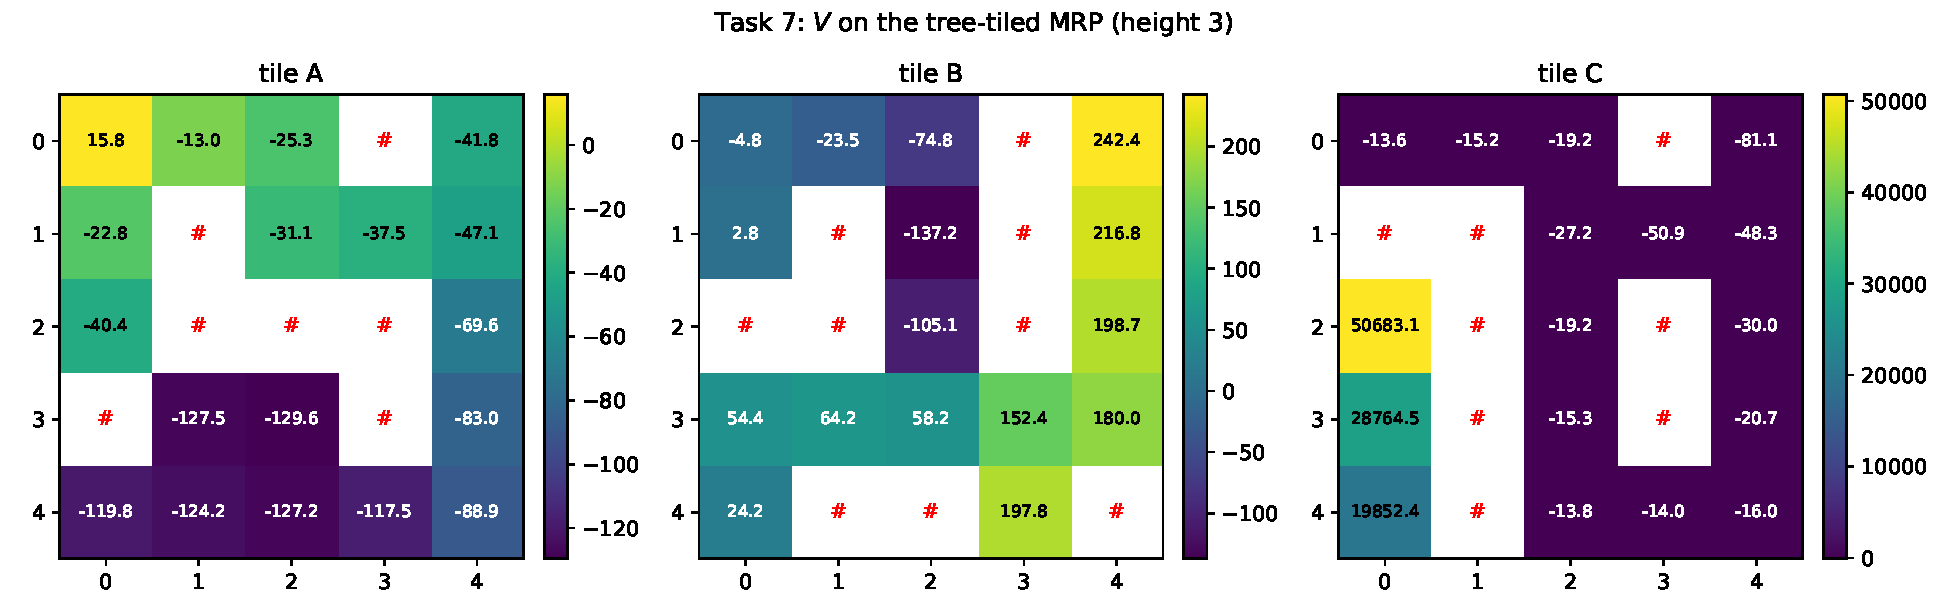
\includegraphics[width=\textwidth]{figures/fig_task7_tiled_values.pdf}
  \caption{\textbf{Task 7.} Iterative-solve $V$ on three tiles
    composed along a binary tree of height 2 (tile $A$ connects to
    tile $B$ which in turn connects to tile $C$). The reward-10\,000
    jackpot in tile $C$ is propagated through the portals into the
    other two tiles; the algorithm correctly finds a path with
    discounted value $\sim\!50{,}683$ starting at the top-left cell of
    $A$.}
  \label{fig:task7}
\end{figure}

Numerically, our height-3 instance has $|S|=51$ and $\text{nnz}(P)=192$;
the iterative solve converges and the optimal value (start-of-$A$) is
pulled up to $\approx 5.07 \times 10^{4}$ through portals to the
jackpot cell of tile $C$, confirming that composition propagates value
across tiles as expected (Figure~\ref{fig:task7}).

\begin{remark}
This construction is a narrow, constructive instance of the
``simplicial complexes of grids'' that the assignment calls out.
Similar Lego-style compositions appear in combinatorial game theory
\citep{conway1976}, where game positions are built from sub-games via
disjunctive sum; and in procedurally-generated RL benchmarks, where a
larger ``meta'' environment is assembled from room-sized tiles. The
key observation is that value iteration remains linear in $\text{nnz}(P)$,
so compositions that add few edges (like portals) scale gracefully
with the number of tiles.
\end{remark}

\section{Task 8 --- Reflection on Markov processes}

\textbf{Advantages.} The Markov property buys three things that the
field has consistently found hard to give up. First, a recursive
Bellman equation whose solution can be attacked by fast linear-algebra
routines or by provably-convergent iteration
\citep{bellman1957,howard1960,puterman1994}. Second, a generative story
where samples $(S_t, A_t, R_{t+1}, S_{t+1})$ are sufficient for
learning, which \emph{enables} model-free algorithms like Q-learning
\citep{watkins1992} and SARSA \citep{rummery1994}. Third, the
state-as-sufficient-statistic framing opens the door to function
approximation via neural networks
\citep{bertsekas1996,mnih2015}.

\textbf{Limitations.} The price is the assumption that the current
state captures everything relevant about the past. Real-world problems
routinely violate this: visual observations are partial
(POMDPs~\citep{kaelbling1998}), relevant history extends beyond the
current frame (motivating recurrent architectures and frame-stacking),
and agents interact with other agents whose policies are
non-stationary (multi-agent RL). Function-approximation schemes can
also introduce artefacts like the ``deadly triad'' of off-policy
bootstrapping with function approximation \citep{thrun1993}.

\textbf{Alternatives.} Several families step outside the plain MDP
formulation while retaining much of its machinery. POMDPs promote the
state to a \emph{belief} over the hidden state and apply the Bellman
equation on the belief space \citep{kaelbling1998}. Semi-Markov
decision processes and options introduce temporal abstraction.
Predictive State Representations replace a latent state with a vector
of predictions about future observations, dispensing with the
hidden-state hypothesis entirely. More radical alternatives include
model-free successor representations, which cache long-run transition
statistics but not a plain $P$; and causal approaches, which impose
intervention invariants alongside (or instead of) Markovianness.

My personal view after this exercise is that the Markov framework is
an almost unreasonably useful abstraction for small, structured
problems --- precisely the regime of grid worlds, where closed-form
Bellman solves are both tractable and insightful. For large
observation spaces the Markov property becomes a \emph{modelling
choice} rather than a true property of the world, and the question
shifts from ``is the MDP correct?'' to ``is the MDP approximation
helpful?'' For procedurally-generated environments like the tree-tiled
worlds of Task 7, the Markov abstraction is natural; for partially
observed, history-dependent, or multi-agent settings, I would want to
move to POMDPs or explicit history models rather than pretend the
Markov property holds.

\section{From Mini-1 to V1 and V2}

The repository accompanying this report also satisfies the V1 and V2
criteria from the course hand-outs. In particular:

\begin{itemize}[leftmargin=2em, itemsep=2pt]
  \item \textbf{Cookiecutter-style layout}: \texttt{src/mini1\_rl/},
    \texttt{scripts/}, \texttt{notebooks/}, \texttt{tests/},
    \texttt{docs/}, \texttt{data/replay\_buffers/}, \texttt{checkpoints/}.
  \item \textbf{V1 item 3 (MDP representation)}: the abstract classes of
    \S\ref{sec:task2} give the agent a place to store and update prior
    beliefs of the transition kernel $P^a$ and reward $\mathcal{R}^a$.
  \item \textbf{V1 item 4 (DP)}: \texttt{PolicyIterationAgent} and
    \texttt{ValueIterationAgent} operate on $V$ \emph{and} $Q$ (the
    helper \texttt{q\_from\_v} lifts $V^\pi$ to $Q^\pi$ in closed form).
  \item \textbf{V1 item 5 (agent framework)}:
    \texttt{BaseAgent} exposes \texttt{train}, \texttt{evaluate},
    \texttt{save}, \texttt{load}; a top-level \texttt{scripts/train.py}
    dispatches on \texttt{--algo} and \texttt{--task}.
  \item \textbf{V2 classical RL}: Monte-Carlo control, $n$-step SARSA,
    backward-view SARSA($\lambda$) with accumulating traces
    \citep{dayan1993}, TD($n$) and TD($\lambda$) for policy evaluation,
    and Q-learning \citep{watkins1992}.
  \item \textbf{V2 replay buffer}: \texttt{buffers/replay.py} provides a
    bounded buffer organised by \texttt{algo/task/freshness}, with a
    rotation CLI in \texttt{scripts/replace\_old\_experience.py}. The
    architecture follows the experience-replay literature
    \citep{lin1992,mnih2015}.
  \item \textbf{V2 NN architectures and DRL}: a minimal
    \texttt{MLP}/\texttt{ConvQNet} module and a full DQN agent
    \citep{mnih2015} with optional EMA target network.
  \item \textbf{V2 utilities}: ASCII rasterization of policies and
    values; saliency via input-gradient $|\partial
    Q_\theta/\partial s|$ \citep{simonyan2014saliency}.
\end{itemize}

Figure~\ref{fig:algo} compares four of the classical agents on the
primary mask with slip $s = 0.1$. Monte-Carlo converges slowly because
every update must propagate through complete episodes; the bootstrapped
agents (SARSA, Q-learning, SARSA($\lambda$)) reach the optimum after
$\sim\!150$ episodes, which matches the $\gamma^k$ contraction budget
one expects from \citet{sutton2018}.

\begin{figure}[h]
  \centering
  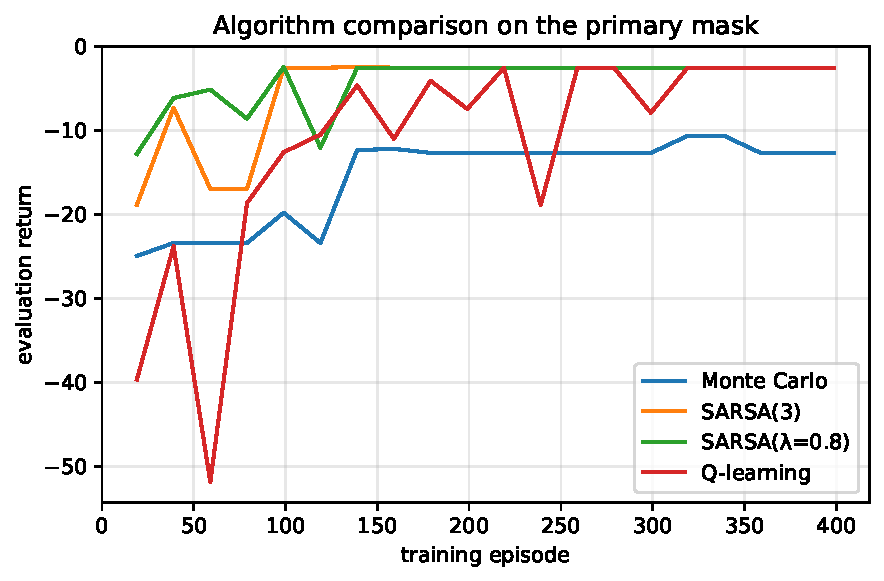
\includegraphics[width=0.7\textwidth]{figures/fig_algo_comparison.pdf}
  \caption{Learning curves for Monte-Carlo, $n$-step SARSA,
    SARSA($\lambda\!=\!0.8$), and Q-learning on the primary mask with
    slip $0.1$ (evaluation return over 20 trajectories, smoothed).
    Bootstrapped agents dominate MC early; all three converge to the
    same final evaluation return.}
  \label{fig:algo}
\end{figure}

\paragraph{Justification for DRL choice.}
V2 asks for one DRL algorithm to be picked and justified. Our
foundation environment is a small tabular gridworld, so the tabular
agents are strictly more sample-efficient than any deep method. We
nevertheless implement \textbf{DQN} because (i) the grid-world
observation is a one-hot vector which maps cleanly onto the
\texttt{MLP} architecture used in \citet{mnih2015}; (ii) off-policy
updates from a replay buffer match the V2 ``organised replay''
requirement; and (iii) DQN is the natural stepping-stone to Double-DQN
\citep{van2016double} and Rainbow once the foundation environment is
scaled to pixel observations. The continuous-control algorithms
(DDPG~\citep{lillicrap2016}, TD3~\citep{fujimoto2018},
SAC~\citep{haarnoja2018}) are not a good fit because our action space
is discrete. Policy-gradient methods
(REINFORCE~\citep{williams1992}, PPO~\citep{schulman2017ppo},
TRPO~\citep{schulman2015}) could be used but their high
variance dwarfs DQN's stability advantage on a problem this small.

\section{Conclusion}

Mini-1 is primarily an exercise in getting the abstractions right,
then letting the Bellman machinery do the rest. Our abstract classes
support plain Markov chains, reward processes, and controlled
processes behind a single policy-induction interface; three
independent solvers agree on the degenerate swap matrix; the
grid-world initializer consumes exactly the 2-D mask the assignment
prescribes; the discount-factor study verifies both the empirical
effect on $V$ and the theoretical $\gamma^k$-contraction rate; and the
optional tree-tiled construction composes up to $2^{h}$ tiles through
portal edges without any 3-D tensors.

\section*{Code and reproducibility}

The entire repository, including the experiments that generated every
figure and table in this report, is accessible as \texttt{mini1-rl}.
The script \texttt{python -m mini1\_rl.experiments.run\_all --out
  docs/report/figures} regenerates all PDFs in the
\texttt{docs/report/figures/} directory, along with a
\texttt{results\_table.json} file containing the raw numeric data
quoted in the text. Unit tests in \texttt{tests/} verify that the
three solvers agree on both the primary mask and the degenerate
example, and that the induced-MRP helper returns the same values as a
directly-constructed MRP on the grid world.

\bibliographystyle{plainnat}
\bibliography{references}

\end{document}
